\subsection{Cancellation}

As of OpenMP 4.0, a thread can be cancelled using a combination of two commands:
\begin{itemize}
    \item \texttt{cancel} construct cancels the innermost enclosing region of the specified type.
    
    In other words, it \textbf{allows us to cancel the current thread}. But be careful! The directive only allows to \textbf{set the cancellation flag to a value of one}. So it is necessary to also use the \texttt{cancellation point} command or the thread must hit a barrier (implicit or explicit).

    The syntax of the \texttt{cancel} construct is as follows:
    \marginpar{
        \href{https://www.openmp.org/spec-html/5.0/openmpsu101.html} {Doc. \faIcon{book}}
    }
    \begin{openmpbox}[: \texttt{pragma omp cancel}]
        \begin{lstlisting}[language=C++, mathescape=true]
#pragma omp cancel $\emph{construct-type-clause}$\end{lstlisting}
        Where \texttt{\emph{construct-type-clause}} is one of the following: \texttt{parallel}, \texttt{sections}, \texttt{for}, \texttt{taskgroup}.
    \end{openmpbox}
    
    \item The \texttt{cancellation point} construct introduces a user-defined cancellation\break point at which implicit or explicit tasks check whether cancellation of the innermost enclosing region of the specified type has been enabled.

    In other words, \textbf{when a thread encounters the cancellation point, the cancellation flag has been checked}. The thread execution is stopped. This is an explicit cancellation request because there are other points where cancellation flag is checked, such as at another cancel region or at a barrier.
    \marginpar{
        \href{https://www.openmp.org/spec-html/5.0/openmpsu102.html\#x134-5350002.18.2} {Doc. \faIcon{book}}
    }
    \begin{openmpbox}[: \texttt{pragma omp cancellation point}]
        \begin{lstlisting}[language=C++]
#pragma omp cancellation point\end{lstlisting}
    \end{openmpbox}
\end{itemize}
Since there is an \textbf{overhead in checking for cancellation}, it can be enabled manually using the \texttt{OMP\_CANCELLATION} environment variable (false by default).

\begin{flushleft}
    \textcolor{Red2}{\faIcon{exclamation-triangle} \textbf{Immediate cancellation is not guaranteed}}
\end{flushleft}
\textbf{OpenMP does not guarantee that cancellation will result in immediate termination}.

\highspace
\begin{flushleft}
    \textcolor{Green3}{\faIcon{check} \textbf{When to use?}}
\end{flushleft}
When there is a \textbf{need to stop the execution}, such as in the \textbf{divide-and-conquer algorithms} (for example, to stop a search when we find the element), or when we \textbf{need to handle some errors}.

\begin{examplebox}[: thread cancellation]
    Assume that from a certain point in our algorithm there are 5 threads alive (including the \emph{master}), and the construct pipeline is as follows.
    \begin{center}
        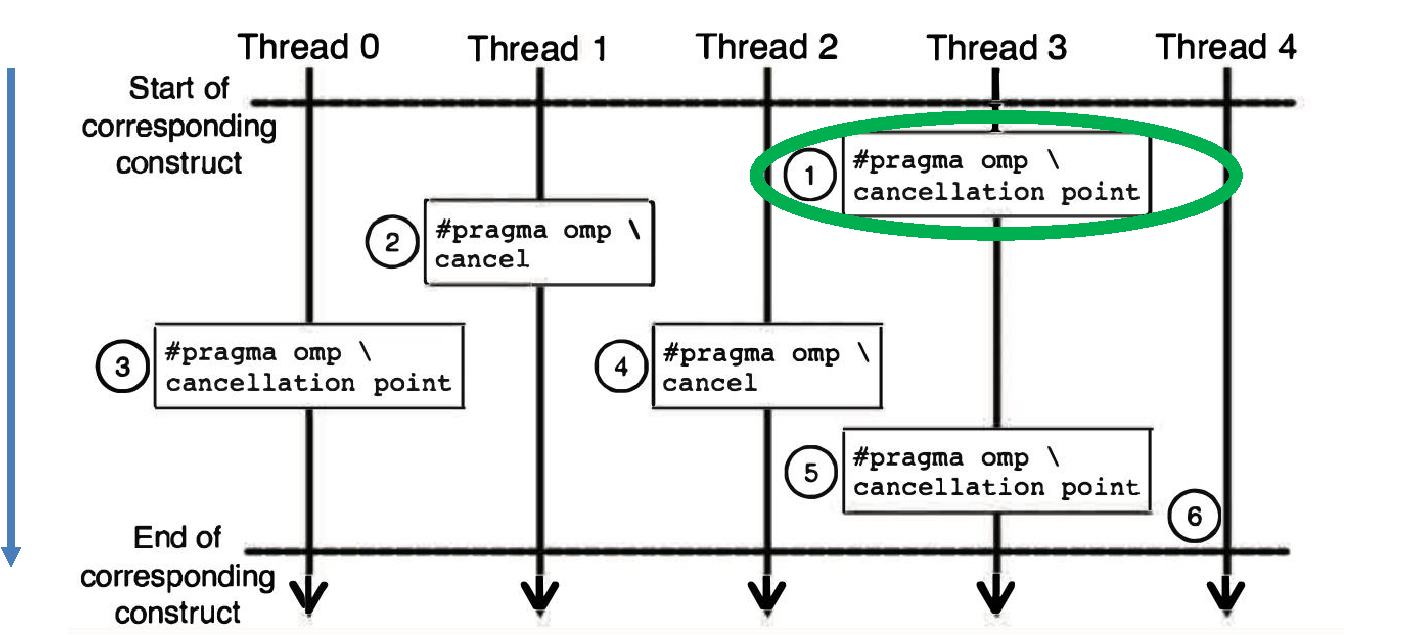
\includegraphics[width=\textwidth]{img/openmp-cancel-1.pdf}
    \end{center}

    Thread 3 hits a cancellation point, but there is no cancel directive before it, so the cancellation flag is set to zero by default and the thread hasn't been broken.
    \begin{center}
        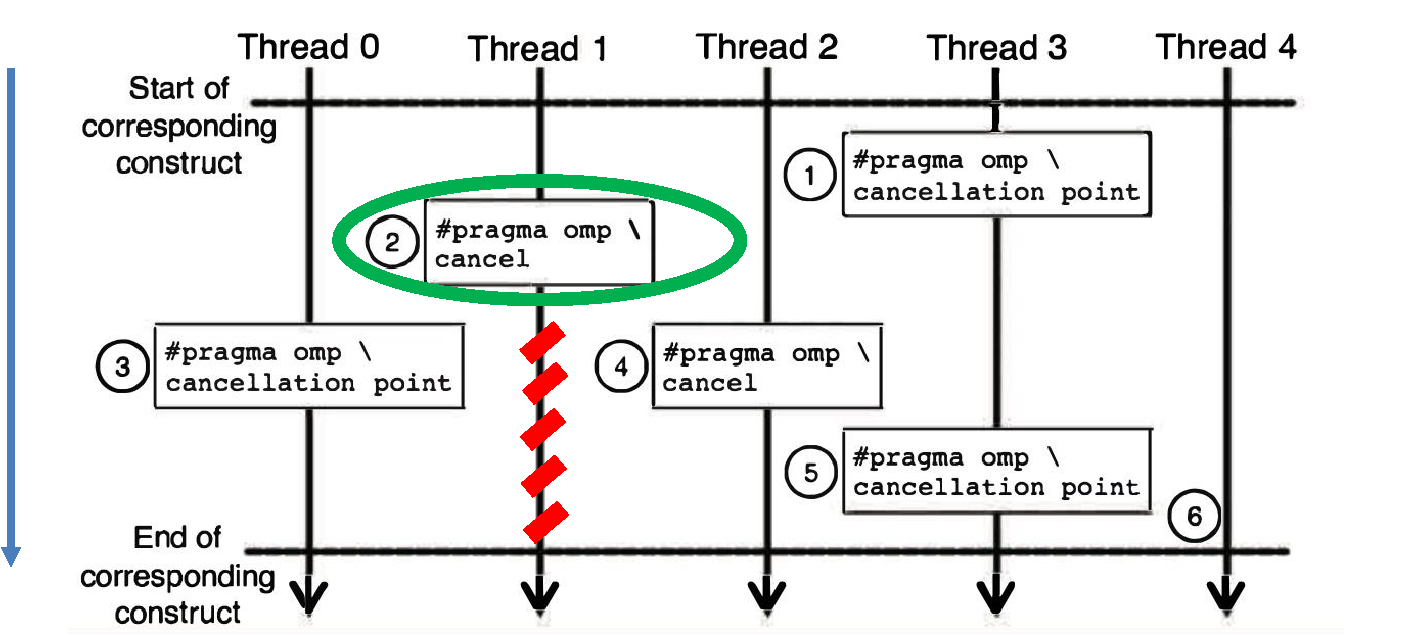
\includegraphics[width=\textwidth]{img/openmp-cancel-2.pdf}
    \end{center}

    Thread 1 requests the cancellation and waits for a synchronization point, such as a barrier or an cancellation point. From that point on, it is idle and waits.
    \begin{center}
        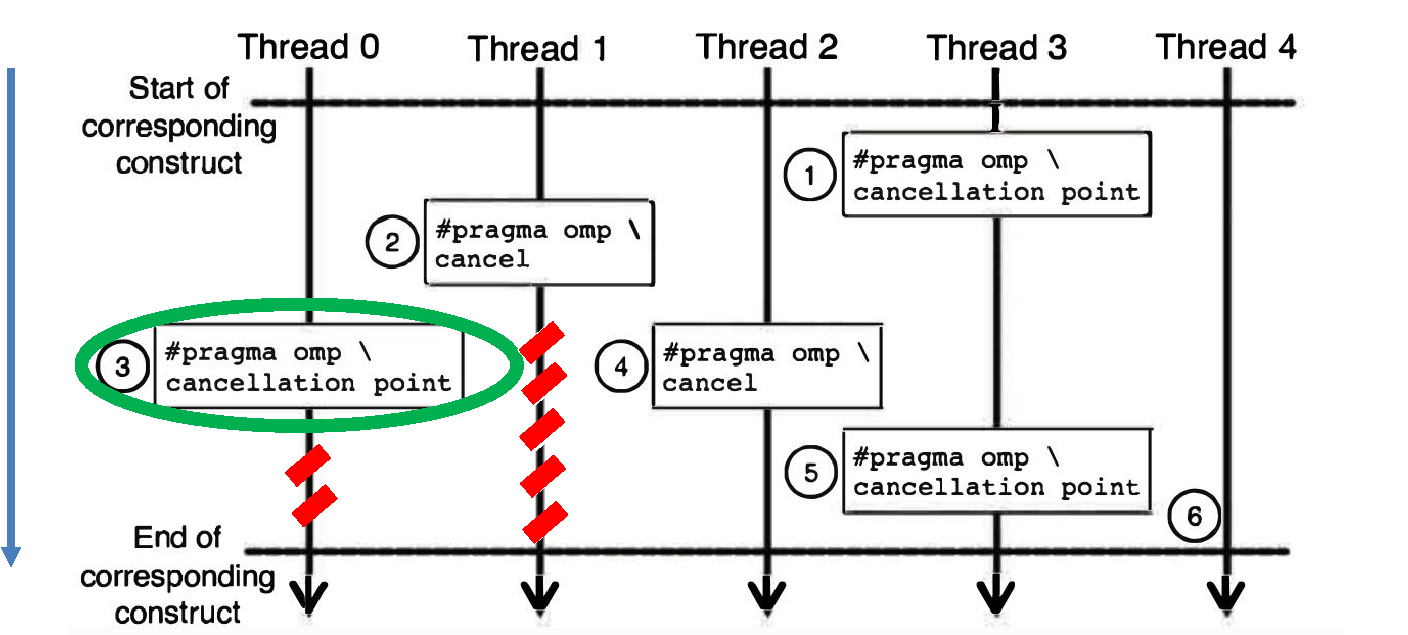
\includegraphics[width=\textwidth]{img/openmp-cancel-3.pdf}
    \end{center}

    Thread 0 calls a cancellation point to check the flag and terminates because thread 1 (last step) has set the cancellation flag to 1. At this point, thread 1, which was waiting for a synchronization point, also terminates.
    \begin{center}
        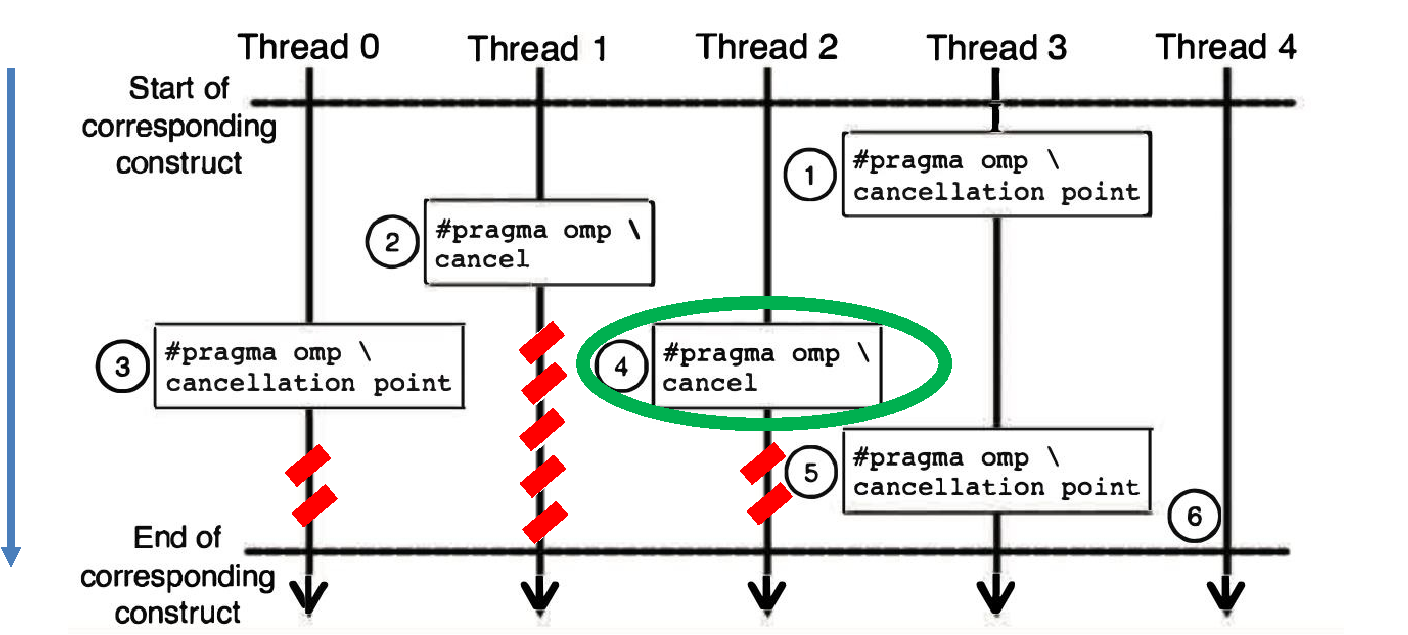
\includegraphics[width=\textwidth]{img/openmp-cancel-4.pdf}
    \end{center}
    
    At the same time, thread 2 is cancelled because the cancel directive checks the cancellation flag first.
    \begin{center}
        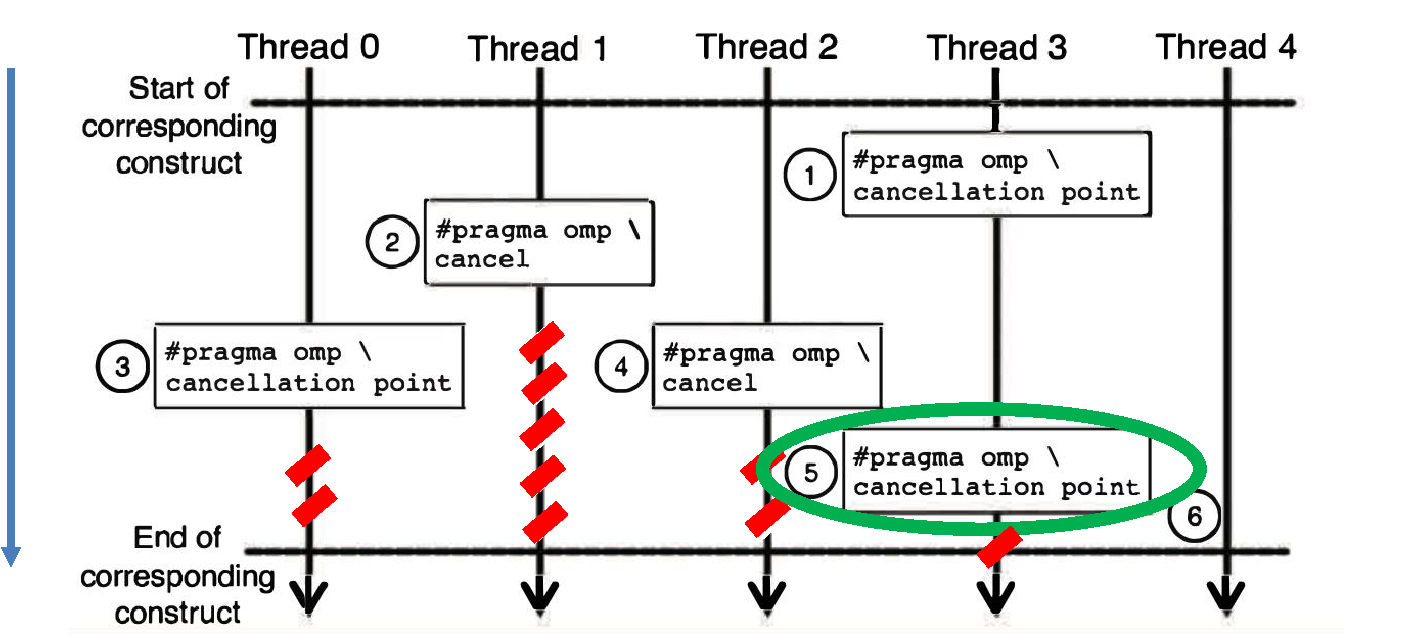
\includegraphics[width=\textwidth]{img/openmp-cancel-5.pdf}
    \end{center}

    At this point the thread 3 has been terminated.
    \begin{center}
        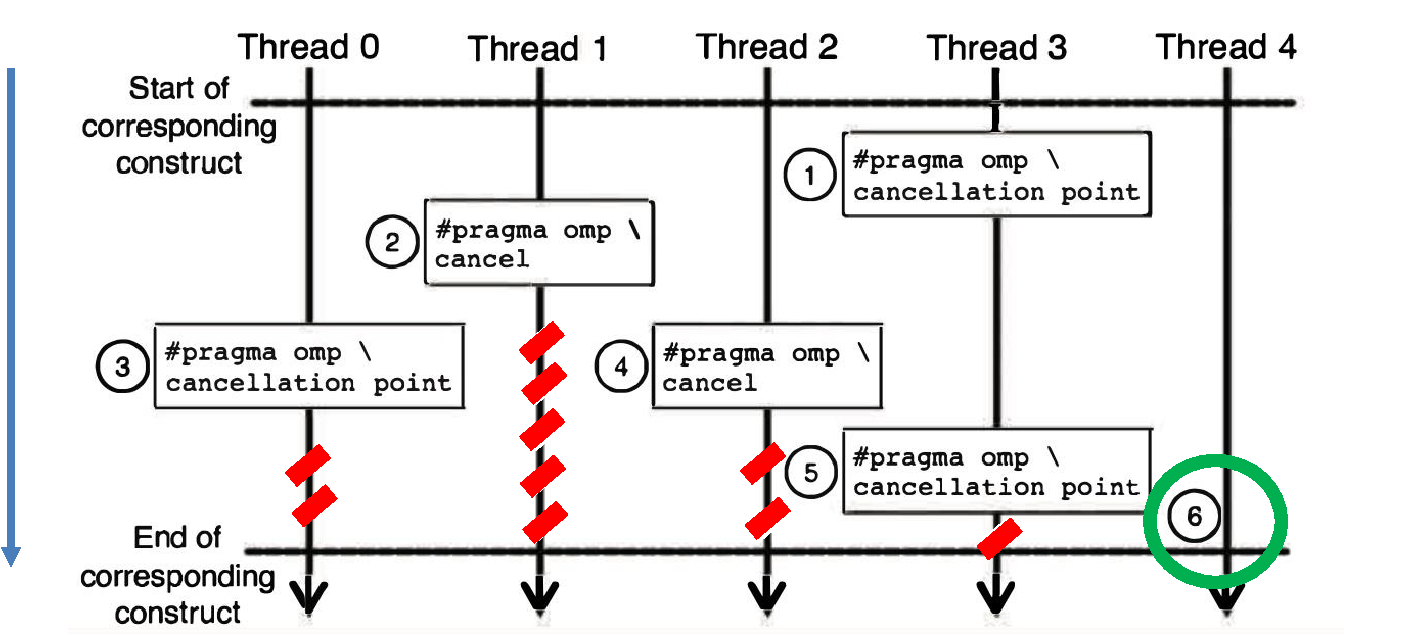
\includegraphics[width=\textwidth]{img/openmp-cancel-6.pdf}
    \end{center}

    Finally, thread 4 never encounters a cancellation point and finishes execution normally.
\end{examplebox}